\documentclass[9pt,a4paper]{article}
\usepackage{iftex}

\ifPDFTeX
  \usepackage[utf8]{inputenc}
  \IfFileExists{l7xenc.def}{%
    \usepackage[L7x,T1]{fontenc}%
  }{%
    \usepackage[T1]{fontenc}%
  }
  \IfFileExists{lithuanian.ldf}{%
    \usepackage[lithuanian]{babel}%
  }{}
  \usepackage{lmodern}
  % Atsarginis UTF-8 lietuviškų raidžių atvaizdavimas, jei kompiliuojama be L7x
  \makeatletter
  \@ifundefined{DeclareUnicodeCharacter}{}{%
    \DeclareUnicodeCharacter{0104}{\k{A}}% Ą
    \DeclareUnicodeCharacter{0105}{\k{a}}% ą
    \DeclareUnicodeCharacter{010C}{\v{C}}% Č
    \DeclareUnicodeCharacter{010D}{\v{c}}% č
    \DeclareUnicodeCharacter{0118}{\k{E}}% Ę
    \DeclareUnicodeCharacter{0119}{\k{e}}% ę
    \DeclareUnicodeCharacter{0116}{\.{E}}% Ė
    \DeclareUnicodeCharacter{0117}{\.{e}}% ė
    \DeclareUnicodeCharacter{012E}{\k{I}}% Į
    \DeclareUnicodeCharacter{012F}{\k{i}}% į
    \DeclareUnicodeCharacter{0160}{\v{S}}% Š
    \DeclareUnicodeCharacter{0161}{\v{s}}% š
    \DeclareUnicodeCharacter{0172}{\k{U}}% Ų
    \DeclareUnicodeCharacter{0173}{\k{u}}% ų
    \DeclareUnicodeCharacter{016A}{\={U}}% Ū
    \DeclareUnicodeCharacter{016B}{\={u}}% ū
    \DeclareUnicodeCharacter{017D}{\v{Z}}% Ž
    \DeclareUnicodeCharacter{017E}{\v{z}}% ž
  }
  \makeatother
\else
  \usepackage{fontspec}
\fi

\usepackage[margin=1.1cm]{geometry}
\usepackage{amsmath,amssymb,amsfonts,mathtools}
\usepackage{multicol}
\usepackage{booktabs}
\usepackage{array}
\usepackage{graphicx}
\usepackage{xcolor}
\usepackage{enumitem}
\usepackage{fancyhdr}
\usepackage{tikz}
\usetikzlibrary{arrows.meta, positioning, shapes.geometric, calc}

\setlist{nosep, leftmargin=*}
\pagestyle{fancy}
\fancyhf{}
\lhead{\textbf{SEM ir Kelių analizė rankomis (S1 formulės ir diagramos)}}
\rhead{VU MIF | Prof. V. Čekanavičius}
\cfoot{\thepage}

\setlength{\columnsep}{14pt}
\setlength{\columnseprule}{0.2pt}

% Tiksli dėžučių pločio kontrolė, apsauganti nuo stulpelio perpildymo
\newcommand{\boxalert}[2]{%
\noindent\fbox{%
\parbox{\dimexpr\linewidth-2\fboxsep-2\fboxrule\relax}{%
\textbf{\textcolor{red!80!black}{#1:}} #2%
}%
}\vspace{1.2mm}%
}

\newcommand{\boxtip}[2]{%
\noindent\fbox{%
\parbox{\dimexpr\linewidth-2\fboxsep-2\fboxrule\relax}{%
\textbf{\textcolor{blue!80!black}{#1:}} #2%
}%
}\vspace{1.2mm}%
}

\title{\vspace{-1.2cm}\Large\textbf{SEM ir Kelių analizė: Formulių ir diagramų konspektas}\\\large Skirta atsiskaitymui ant popieriaus (S1) pagal vadovėlį\vspace{-0.5cm}}
\author{Pagal prof. V. Čekanavičiaus „Statistika ir jos taikymai III“ ir paskaitų pavyzdžius}
\date{}

\begin{document}
\maketitle
\thispagestyle{fancy}

\begin{multicols*}{2}

\section{Pagrindinės sąvokos ir diagramų elementai}
Atsiskaityme rankomis kintamieji beveik visada laikomi \textbf{standartizuotais}:
\begin{equation*}
    E[X] = 0, \quad \text{Var}(X) = 1 \implies \text{Cov}(X, Y) = \text{Cor}(X, Y) = r_{XY}
\end{equation*}

\subsection{Kintamųjų tipai diagramoje}
\begin{itemize}
    \item \textbf{Egzogeninis} ($X, \xi$): nepriklausomas kintamasis. Į jį \textbf{neįeina jokia vienkryptė rodyklė} (iš jo rodyklės tik išeina).
    \begin{itemize}
        \item \textit{Savybė}: \textbf{neturi liekamosios paklaidos} $e$.
        \item \textit{Vertinama}: jo dispersija ir tarpusavio kovariacijos/koreliacijos su kitais egzogeniniais kintamaisiais.
    \end{itemize}
    \item \textbf{Endogeninis} ($Y, \eta$): priklausomas kintamasis. Į jį \textbf{įeina bent viena vienkryptė rodyklė} $\to$.
    \begin{itemize}
        \item \textit{Savybė}: \textbf{kiekvienas endogeninis kintamasis privalo turėti liekamąją paklaidą} ($e, \delta, d$).
        \item \textit{Vertinama}: įeinančių kelių koeficientai ir paklaidos dispersija $\text{Var}(e)$.
    \end{itemize}
    \item \textbf{Stebimi kintamieji} (indikatoriai): žymimi \textbf{stačiakampiais}.
    \item \textbf{Latentiniai faktoriai}: žymimi \textbf{ovalais / elipsėmis}.
    \item \textbf{Liekamosios paklaidos}: žymimos \textbf{mažais apskritimais}.
\end{itemize}

\subsection{Ryšių tipai kelių diagramose}
\begin{itemize}
    \item $X \xrightarrow{\beta} Y$: tiesioginė įtaka (kelio / regresijos svoris $\beta$).
    \item $X \xleftrightarrow{r} Y$: dvipusė lankinė rodyklė (koreliacija arba kovariacija). Priežastinis ryšys nenurodomas.
    \item $e \to Y$: liekamoji paklaida (kelio svoris fiksuojamas $1$, o vertinama dispersija $\text{Var}(e)$).
\end{itemize}

\subsection{Latentinių kintamųjų skalės fiksavimas}
Latentiniai faktoriai neturi matavimo vienetų, todėl modeliui identifikuoti būtina fiksuoti skalę vienu iš 2 būdų:
\begin{enumerate}
    \item \textbf{Žymimasis indikatorius} (\textit{marker variable}): vieno indikatoriaus kelio svoris fiksuojamas $\lambda_1 = 1$.
    \item \textbf{Standartizuotas faktorius}: fiksuojama paties latentinio faktoriaus dispersija $\text{Var}(\xi) = 1$.
\end{enumerate}

\section{Wright'o kelių sekimo taisyklės (\textit{Tracing rules})}
Koreliacija tarp dviejų standartizuotų kintamųjų $X$ ir $Y$ lygi visų \textbf{leistinų jungiančių kelių} sandaugų sumai:
\begin{equation*}
    \text{Cor}(X, Y) = \sum_{\text{visi leistini keliai } p} \prod_{k \in p} w_k
\end{equation*}

\boxalert{4 Wright'o taisyklės leistinam keliui}{%
\begin{enumerate}
    \item \textbf{Nėra kilpų}: kelias negali praeiti pro tą patį kintamąjį daugiau nei 1 kartą.
    \item \textbf{Draudžiama $\to \leftarrow$}: negalima eiti rodykle pirmyn, o po to atgal! Tai susidūrimo taškas (\textit{collider} / bendra pasekmė).
    \item \textbf{Leidžiama $\leftarrow \to$}: galima eiti atgal, o po to pirmyn! Tai bendra priežastis (\textit{common cause}).
    \item \textbf{Ne daugiau 1 koreliacijos}: kelyje leidžiamas daugiausiai vienas dvipusis lankas $\leftrightarrow$.
\end{enumerate}
}

\section{Poveikių išskaidymas (\textit{Effect decomposition})}
Vieno kintamojo $X$ ryšys su kitu kintamuoju $Y$ išskaidomas į dedamąsias:
\begin{itemize}
    \item \textbf{Tiesioginis poveikis} (\textit{Direct effect, DE}): kelio koeficientas tiesiogiai iš $X \to Y$.
    \item \textbf{Netiesioginis poveikis} (\textit{Indirect effect, IE}): kelių per visus tarpinius kintamuosius koeficientų sandaugų suma ($X \to M_1 \to \dots \to Y$).
    \item \textbf{Bendrasis priežastinis poveikis} (\textit{Total causal effect, TE}):
    \begin{equation*}
        \text{TE} = \text{DE} + \text{IE}
    \end{equation*}
    \item \textbf{Neanalizuojamas poveikis} (\textit{Unanalyzed}): atsiranda dėl egzogeninių kintamųjų tarpusavio koreliacijos (kelyje yra dvipusis lankas $\leftrightarrow$).
    \item \textbf{Iškraipytas poveikis} (\textit{Spurious / Distorted}): atsiranda dėl bendros trečio kintamojo priežasties ($\leftarrow Z \to$).
\end{itemize}
\begin{equation*}
    \text{Bendra koreliacija } r_{XY} = \text{TE} + \text{Neanalizuojamas} + \text{Iškraipytas}
\end{equation*}

\section{Modelio identifikavimas ir laisvės laipsniai}
\subsection{Duomenų taškų skaičius ($p^*$)}
\begin{itemize}
    \item Kai žinoma \textbf{kovariacijų matrica} ($k$ kintamųjų):
    \begin{equation*}
        p^* = \frac{k(k + 1)}{2} \quad (\text{apima } k \text{ dispersijų})
    \end{equation*}
    \item Kai žinoma \textbf{koreliacijų matrica} (standartizuota):
    \begin{equation*}
        p^* = \frac{k(k - 1)}{2} \quad (\text{įstrižainėje vienetai})
    \end{equation*}
\end{itemize}

\subsection{Laisvės laipsniai ($df$)}
Tarkime, kad modelyje laisvai vertinamų parametrų skaičius yra $q$:
\begin{equation*}
    df = p^* - q
\end{equation*}
\begin{itemize}
    \item $df > 0$: \textbf{Perteklinis} (\textit{Over-identified}). Modelį galima tikrinti $\chi^2$ ir suderinamumo indeksais.
    \item $df = 0$: \textbf{Tiksliai identifikuojamas / pilnasis} (\textit{Just-identified}). $\hat{\Sigma} = S$, $\chi^2 = 0$, tobulas sutapimas garantuotas matematiškai.
    \item $df < 0$: \textbf{Neidentifikuojamas} (\textit{Under-identified}). Parametrų rasti neįmanoma (trūksta lygčių).
\end{itemize}

\subsection{Identifikavimo taisyklės}
\begin{enumerate}
    \item \textbf{$t$-taisyklė} (būtina sąlyga): $q \le p^*$.
    \item \textbf{Rekursyvumo taisyklė}: jei modelio diagramoje \textbf{nėra grįžtamųjų ciklų} ir \textbf{liekamosios paklaidos nekoreliuoja}, modelis garantuotai identifikuojamas.
    \item \textbf{CFA taisyklė}:
    \begin{itemize}
        \item 1 faktoriaus modelis: reikia bent \textbf{3 indikatorių}.
        \item $\ge 2$ koreliuojančių faktorių: reikia bent \textbf{2 indikatorių} kiekvienam faktoriui.
    \end{itemize}
\end{enumerate}

\section{Paklaidų dispersijos $\text{Var}(e)$ ir $R^2$ rankomis}
Standartizuotam endogeniniam kintamajam $Y$:
\begin{equation*}
    \text{Var}(Y) = 1 = R_Y^2 + \text{Var}(e_Y) \implies \text{Var}(e_Y) = 1 - R_Y^2
\end{equation*}
Determinacijos koeficientas $R_Y^2$:
\begin{equation*}
    R_Y^2 = \sum_j \beta_j \cdot \text{Cor}(X_j, Y)
\end{equation*}
Pvz., jei $Y = a X_1 + b X_2 + e_Y$:
\begin{align*}
    R_Y^2 &= a \cdot \text{Cor}(X_1, Y) + b \cdot \text{Cor}(X_2, Y) \\
    \text{Var}(e_Y) &= 1 - \big(a \cdot r_{1Y} + b \cdot r_{2Y}\big)
\end{align*}

\section{Greitoji formulė 2x2 lygčių sistemoms (Egzamino formulė)}
\boxalert{Kramerio formulė 2x2 sistemai}{%
Kelių analizėje nuolat atsiranda sistema:
\begin{equation*}
    \begin{cases} \beta_1 + r \beta_2 = r_{1Y} \\ r \beta_1 + \beta_2 = r_{2Y} \end{cases}, \quad \text{kur } r = \text{Cor}(X_1, X_2)
\end{equation*}
Determinantas: $D = 1 - r^2$. Sprendiniai gaunami iš karto:
\begin{align*}
    \beta_1 &= \frac{r_{1Y} - r \cdot r_{2Y}}{1 - r^2} \\
    \beta_2 &= \frac{r_{2Y} - r \cdot r_{1Y}}{1 - r^2}
\end{align*}
Sutaupo skaičiavimo laiką ir apsaugo nuo aritmetinių klaidų!
}

\section{SEM matricinė struktūra (LISREL ir 3.3.9 pav.)}
Šiame skyriuje pateikiama tiksli vadovėlio \textbf{3.3.9 pav.} diagrama ir jos užrašymas LISREL matricomis pagal pavyzdį 3.3.4.

\begin{center}
\resizebox{0.95\columnwidth}{!}{%
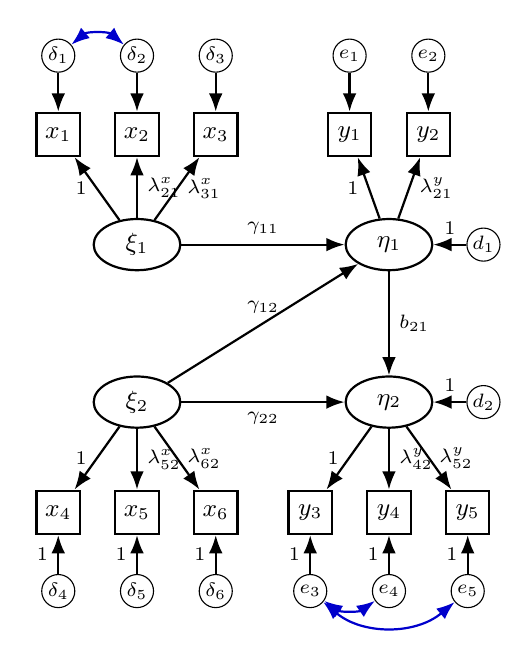
\begin{tikzpicture}[
  >=Latex,
  latent/.style={ellipse, draw=black, thick, minimum width=1.1cm, minimum height=0.65cm, inner sep=1pt, font=\small},
  manifest/.style={rectangle, draw=black, thick, minimum size=0.55cm, inner sep=1pt, font=\small},
  error/.style={circle, draw=black, minimum size=0.42cm, inner sep=0.5pt, font=\scriptsize},
  patharrow/.style={->, thick},
  covarrow/.style={<->, bend left=30, thick, color=blue!80!black}
]
  % Latents xi
  \node[latent] (xi1) at (1.2, 3.2) {$\xi_1$};
  \node[latent] (xi2) at (1.2, 1.2) {$\xi_2$};

  % Manifest x for xi1
  \node[manifest] (x1) at (0.2, 4.6) {$x_1$};
  \node[manifest] (x2) at (1.2, 4.6) {$x_2$};
  \node[manifest] (x3) at (2.2, 4.6) {$x_3$};

  % Errors delta for x1, x2, x3
  \node[error] (d1) at (0.2, 5.6) {$\delta_1$};
  \node[error] (d2) at (1.2, 5.6) {$\delta_2$};
  \node[error] (d3) at (2.2, 5.6) {$\delta_3$};

  % Manifest x for xi2
  \node[manifest] (x4) at (0.2, -0.2) {$x_4$};
  \node[manifest] (x5) at (1.2, -0.2) {$x_5$};
  \node[manifest] (x6) at (2.2, -0.2) {$x_6$};

  % Errors delta for x4, x5, x6
  \node[error] (d4) at (0.2, -1.2) {$\delta_4$};
  \node[error] (d5) at (1.2, -1.2) {$\delta_5$};
  \node[error] (d6) at (2.2, -1.2) {$\delta_6$};

  % Latents eta
  \node[latent] (eta1) at (4.4, 3.2) {$\eta_1$};
  \node[latent] (eta2) at (4.4, 1.2) {$\eta_2$};

  % Manifest y for eta1
  \node[manifest] (y1) at (3.9, 4.6) {$y_1$};
  \node[manifest] (y2) at (4.9, 4.6) {$y_2$};

  % Errors e for y1, y2
  \node[error] (e1) at (3.9, 5.6) {$e_1$};
  \node[error] (e2) at (4.9, 5.6) {$e_2$};

  % Manifest y for eta2
  \node[manifest] (y3) at (3.4, -0.2) {$y_3$};
  \node[manifest] (y4) at (4.4, -0.2) {$y_4$};
  \node[manifest] (y5) at (5.4, -0.2) {$y_5$};

  % Errors e for y3, y4, y5
  \node[error] (e3) at (3.4, -1.2) {$e_3$};
  \node[error] (e4) at (4.4, -1.2) {$e_4$};
  \node[error] (e5) at (5.4, -1.2) {$e_5$};

  % Disturbances d1, d2
  \node[error] (zeta1) at (5.6, 3.2) {$d_1$};
  \node[error] (zeta2) at (5.6, 1.2) {$d_2$};

  % Measurement arrows xi -> x
  \draw[patharrow] (xi1) -- node[left, font=\scriptsize] {$1$} (x1);
  \draw[patharrow] (xi1) -- node[right, font=\scriptsize] {$\lambda_{21}^x$} (x2);
  \draw[patharrow] (xi1) -- node[right, font=\scriptsize] {$\lambda_{31}^x$} (x3);

  \draw[patharrow] (xi2) -- node[left, font=\scriptsize] {$1$} (x4);
  \draw[patharrow] (xi2) -- node[right, font=\scriptsize] {$\lambda_{52}^x$} (x5);
  \draw[patharrow] (xi2) -- node[right, font=\scriptsize] {$\lambda_{62}^x$} (x6);

  % Delta arrows -> x
  \draw[patharrow] (d1) -- (x1);
  \draw[patharrow] (d2) -- (x2);
  \draw[patharrow] (d3) -- (x3);
  \draw[patharrow] (d4) -- node[left, font=\scriptsize] {$1$} (x4);
  \draw[patharrow] (d5) -- node[left, font=\scriptsize] {$1$} (x5);
  \draw[patharrow] (d6) -- node[left, font=\scriptsize] {$1$} (x6);

  % Correlated delta
  \draw[covarrow] (d1) to[bend left=40] (d2);

  % Measurement arrows eta -> y
  \draw[patharrow] (eta1) -- node[left, font=\scriptsize] {$1$} (y1);
  \draw[patharrow] (eta1) -- node[right, font=\scriptsize] {$\lambda_{21}^y$} (y2);

  \draw[patharrow] (eta2) -- node[left, font=\scriptsize] {$1$} (y3);
  \draw[patharrow] (eta2) -- node[right, font=\scriptsize] {$\lambda_{42}^y$} (y4);
  \draw[patharrow] (eta2) -- node[right, font=\scriptsize] {$\lambda_{52}^y$} (y5);

  % Errors e arrows -> y
  \draw[patharrow] (e1) -- (y1);
  \draw[patharrow] (e2) -- (y2);
  \draw[patharrow] (e3) -- node[left, font=\scriptsize] {$1$} (y3);
  \draw[patharrow] (e4) -- node[left, font=\scriptsize] {$1$} (y4);
  \draw[patharrow] (e5) -- node[left, font=\scriptsize] {$1$} (y5);

  % Correlated e
  \draw[<->, thick, color=blue!80!black, bend right=35] (e3) to (e4);
  \draw[<->, thick, color=blue!80!black, bend right=40] (e3) to (e5);

  % Disturbance arrows -> eta
  \draw[patharrow] (zeta1) -- node[above, font=\scriptsize] {$1$} (eta1);
  \draw[patharrow] (zeta2) -- node[above, font=\scriptsize] {$1$} (eta2);

  % Structural paths between latents
  \draw[patharrow] (xi1) -- node[above, font=\scriptsize] {$\gamma_{11}$} (eta1);
  \draw[patharrow] (xi2) -- node[above, font=\scriptsize] {$\gamma_{12}$} (eta1);
  \draw[patharrow] (xi2) -- node[below, font=\scriptsize] {$\gamma_{22}$} (eta2);
  \draw[patharrow] (eta1) -- node[right, font=\scriptsize] {$b_{21}$} (eta2);
\end{tikzpicture}
}%
\end{center}
\vspace{-2mm}
\noindent{\footnotesize\textbf{3.3.9 pav.} Klasikinio SEM modelio diagrama (Čekanavičius, p. 207).}

\subsection{LISREL lygčių sistema}
\begin{align*}
    \text{Struktūrinis: } &\eta = B \eta + \Gamma \xi + d \\
    \text{Matavimas } (Y): &Y = \Lambda_y \eta + e \\
    \text{Matavimas } (X): &X = \Lambda_x \xi + \delta
\end{align*}

\subsection{Kaip iš diagramos užrašyti matricas:}
\begin{enumerate}
    \item \textbf{Stulpeliai} atitinka faktorius, iš kurių išeina rodyklė.
    \item \textbf{Eilutės} atitinka kintamuosius, į kuriuos įeina rodyklė.
    \item Jei rodyklės nėra $\to 0$; jei fiksuotas $\to 1$; jei laisvas $\to \lambda, \gamma, b$.
\end{enumerate}

\textbf{3.3.9 pav. atitinkančios matricos}:
\begin{equation*}
    B = \begin{pmatrix} 0 & 0 \\ b_{21} & 0 \end{pmatrix}, \quad \Gamma = \begin{pmatrix} \gamma_{11} & \gamma_{12} \\ 0 & \gamma_{22} \end{pmatrix}
\end{equation*}
\begin{equation*}
    \Lambda_y = \begin{pmatrix} 1 & 0 \\ \lambda_{21}^y & 0 \\ 0 & 1 \\ 0 & \lambda_{42}^y \\ 0 & \lambda_{52}^y \end{pmatrix}, \quad \Lambda_x = \begin{pmatrix} 1 & 0 \\ \lambda_{21}^x & 0 \\ \lambda_{31}^x & 0 \\ 0 & 1 \\ 0 & \lambda_{52}^x \\ 0 & \lambda_{62}^x \end{pmatrix}
\end{equation*}
\textbf{Paklaidų kovariacijų matricos}:
\begin{itemize}
    \item $\Theta_\delta$ ($6\times 6$): įstrižainėje $D(\delta_i)$, o elementai $(1,2)$ ir $(2,1)$ yra $\text{Cov}(\delta_1, \delta_2)$ dėl lanko tarp $\delta_1 \leftrightarrow \delta_2$.
    \item $\Theta_\epsilon$ ($5\times 5$): įstrižainėje $D(e_i)$, o pozicijose $(3,4), (3,5)$ yra $\text{Cov}(e_3, e_4)$ ir $\text{Cov}(e_3, e_5)$.
    \item $\Phi = \text{diag}(D\xi_1, D\xi_2)$, \quad $\Psi = \text{diag}(Dd_1, Dd_2)$.
\end{itemize}

\section{Mokinio savybių modeliai (3.3.7 pav.)}
Vadovėlio 3.3.7 pav. nagrinėjami 3 Multitrait-Multimethod (MTMM) modelio variantai:

\begin{enumerate}
    \item \textbf{a) MTMM modelis}:
    \begin{itemize}
        \item Viršuje 3 bruožų faktoriai: $\text{Patr}, \text{Gab}, \text{Lyd}$ (su lankais $\leftrightarrow$).
        \item Apačioje 3 metodų faktoriai: $\text{Mok}, \text{Tėv}, \text{Klas}$ (su lankais $\leftrightarrow$).
        \item Kiekvienas iš 9 indikatorių ($p_m, g_m, \dots, v_k$) turi \textbf{dvi įeinančias rodykles}: vieną iš savo bruožo ir vieną iš vertinimo metodo.
    \end{itemize}
    \item \textbf{b) CTCU modelis} (\textit{Correlated Trait -- Correlated Uniqueness}):
    \begin{itemize}
        \item Metodų faktoriai apačioje \textbf{pašalinami}.
        \item Vietoj jų įvedami \textbf{koreliuojančių liekamųjų paklaidų lankai} tarp to paties vertinimo būdo: $e_1 \leftrightarrow e_2 \leftrightarrow e_3$ (mokytojų), $e_4 \leftrightarrow e_5 \leftrightarrow e_6$ (tėvų), $e_7 \leftrightarrow e_8 \leftrightarrow e_9$ (klasės).
    \end{itemize}
    \item \textbf{c) CT modelis} (\textit{Correlated Trait only}):
    \begin{itemize}
        \item Tik bruožų faktoriai viršuje, o liekamosios paklaidos tarpusavyje \textbf{nekoreliuoja}.
    \end{itemize}
\end{enumerate}
\boxtip{Egzamino esmė}{%
Jei CTCU tinka žymiai geriau nei CT modelis $\implies$ vertinimo metodas daro statistiškai reikšmingą įtaką matavimams!
}

\section{1 Pavyzdys: Rasti ryšių reikšmes (Žalia lenta)}
\textbf{Sąlyga}:
Duota kelio diagrama tarp 4 kintamųjų $A, B, C, D$:

\begin{center}
\resizebox{0.65\columnwidth}{!}{%
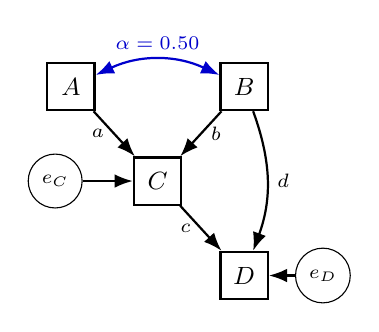
\begin{tikzpicture}[
  >=Latex,
  obs/.style={rectangle, draw=black, thick, minimum size=0.6cm, font=\small},
  err/.style={circle, draw=black, minimum size=0.45cm, font=\scriptsize}
]
  \node[obs] (A) at (0, 2) {$A$};
  \node[obs] (B) at (2.2, 2) {$B$};
  \node[obs] (C) at (1.1, 0.8) {$C$};
  \node[obs] (D) at (2.2, -0.4) {$D$};

  \node[err] (eC) at (-0.2, 0.8) {$e_C$};
  \node[err] (eD) at (3.2, -0.4) {$e_D$};

  \draw[<->, thick, color=blue!80!black, bend left=25] (A) to node[above, font=\scriptsize] {$\alpha=0.50$} (B);
  \draw[->, thick] (A) -- node[left, font=\scriptsize] {$a$} (C);
  \draw[->, thick] (B) -- node[right, font=\scriptsize] {$b$} (C);
  \draw[->, thick] (C) -- node[left, font=\scriptsize] {$c$} (D);
  \draw[->, thick] (B) to[bend left=20] node[right, font=\scriptsize] {$d$} (D);
  \draw[->, thick] (eC) -- (C);
  \draw[->, thick] (eD) -- (D);
\end{tikzpicture}
}%
\end{center}

Duota koreliacijų matrica:
\begin{center}
\begin{tabular}{c|cccc}
 & $A$ & $B$ & $C$ & $D$ \\
\hline
$A$ & 1 & 0.50 & 0.60 & 0.20 \\
$B$ & & 1 & 0.70 & 0.25 \\
$C$ & & & 1 & 0.30 \\
$D$ & & & & 1 \\
\end{tabular}
\end{center}

\textbf{Sprendimas žingsnis po žingsnio}:

\textbf{1 žingsnis}: Randame $\alpha$.\\
Tarp egzogeninių kintamųjų $A$ ir $B$ yra tik dvipusis lankas:
\begin{equation*}
    \alpha = \text{Cor}(A, B) = 0.50
\end{equation*}

\textbf{2 žingsnis}: Randame $a$ ir $b$ (kintamajam $C$).\\
Struktūrinė lygtis: $C = a A + b B + e_C$.\\
Pagal Wright'o taisykles:
\begin{align*}
    \text{Cor}(A, C) &= a + \alpha b = a + 0.5 b = 0.60 \\
    \text{Cor}(B, C) &= \alpha a + b = 0.5 a + b = 0.70
\end{align*}
Taikome greitąją 2x2 formulę ($r = 0.5$, $1 - r^2 = 0.75$):
\begin{align*}
    a &= \frac{0.60 - 0.5 \cdot 0.70}{0.75} = \frac{0.25}{0.75} = \frac{1}{3} \approx 0.333 \\
    b &= \frac{0.70 - 0.5 \cdot 0.60}{0.75} = \frac{0.40}{0.75} = \frac{8}{15} \approx 0.533
\end{align*}

\textbf{3 žingsnis}: Randame $c$ ir $d$ (kintamajam $D$).\\
Struktūrinė lygtis: $D = c C + d B + e_D$.\\
Užrašome $D$ koreliacijas su $B$ ir $A$:
\begin{align*}
    \text{Cor}(B, D) &= c \cdot \text{Cor}(B, C) + d \cdot \text{Cor}(B, B) \\
    &= 0.70 c + 1.0 d = 0.25 \\
    \text{Cor}(A, D) &= c \cdot \text{Cor}(A, C) + d \cdot \text{Cor}(A, B) \\
    &= 0.60 c + 0.50 d = 0.20
\end{align*}
Padauginame antrąją lygtį iš 2: $1.20 c + d = 0.40$. Atimame pirmąją lygtį:
\begin{equation*}
    (1.20 c + d) - (0.70 c + d) = 0.40 - 0.25 \implies 0.50 c = 0.15 \implies c = 0.30
\end{equation*}
Įstatome $c = 0.30$ į pirmąją lygtį:
\begin{equation*}
    d = 0.25 - 0.70(0.30) = 0.25 - 0.21 = 0.04
\end{equation*}

\textbf{Galutiniai ryšių koeficientai}:
\begin{align*}
    \alpha &= 0.50, \quad a = 1/3 \approx 0.333, \\
    b &= 8/15 \approx 0.533, \quad c = 0.30, \quad d = 0.04
\end{align*}

\textbf{Liekamųjų paklaidų dispersijos}:
\begin{align*}
    \text{Var}(e_C) &= 1 - (a \cdot r_{AC} + b \cdot r_{BC}) \\
    &= 1 - (0.20 + 0.3733) = 0.4267 \\
    \text{Var}(e_D) &= 1 - (c \cdot r_{CD} + d \cdot r_{BD}) \\
    &= 1 - (0.09 + 0.01) = 0.90
\end{align*}

\section{2 Pavyzdys: Užrašyti visas koreliacijas (Baltas ekranas)}
\textbf{Sąlyga}:
Pradinis šakninis kintamasis $*$ nukreipia rodykles į $A, B, C$:

\begin{center}
\resizebox{0.75\columnwidth}{!}{%
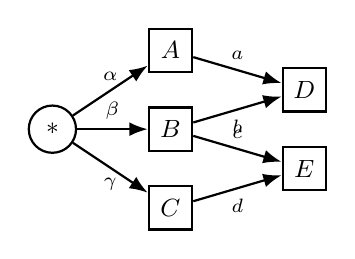
\begin{tikzpicture}[
  >=Latex,
  obs/.style={rectangle, draw=black, thick, minimum size=0.55cm, font=\small},
  rootnode/.style={circle, draw=black, thick, minimum size=0.6cm, font=\small}
]
  \node[rootnode] (X) at (0, 1.2) {$*$};
  \node[obs] (A) at (1.5, 2.2) {$A$};
  \node[obs] (B) at (1.5, 1.2) {$B$};
  \node[obs] (C) at (1.5, 0.2) {$C$};
  \node[obs] (D) at (3.2, 1.7) {$D$};
  \node[obs] (E) at (3.2, 0.7) {$E$};

  \draw[->, thick] (X) -- node[above, font=\scriptsize] {$\alpha$} (A);
  \draw[->, thick] (X) -- node[above, font=\scriptsize] {$\beta$} (B);
  \draw[->, thick] (X) -- node[below, font=\scriptsize] {$\gamma$} (C);

  \draw[->, thick] (A) -- node[above, font=\scriptsize] {$a$} (D);
  \draw[->, thick] (B) -- node[below, font=\scriptsize] {$b$} (D);
  \draw[->, thick] (B) -- node[above, font=\scriptsize] {$c$} (E);
  \draw[->, thick] (C) -- node[below, font=\scriptsize] {$d$} (E);
\end{tikzpicture}
}%
\end{center}

\textbf{Visų koreliacijų išvedimas pagal Wright'o taisykles}:

\subsection{1. Koreliacijos su šakniniu kintamuoju $*$}
\begin{align*}
    \text{Cor}(*, A) &= \alpha, \quad \text{Cor}(*, B) = \beta, \quad \text{Cor}(*, C) = \gamma \\
    \text{Cor}(*, D) &= \alpha a + \beta b \\
    \text{Cor}(*, E) &= \beta c + \gamma d
\end{align*}

\subsection{2. Koreliacijos tarp pirmojo lygio ($A, B, C$)}
Jungiasi per bendrą priežastį $*$ ($\leftarrow * \to$):
\begin{equation*}
    \text{Cor}(A, B) = \alpha \beta, \quad \text{Cor}(A, C) = \alpha \gamma, \quad \text{Cor}(B, C) = \beta \gamma
\end{equation*}

\subsection{3. Koreliacijos tarp lygmenų}
\textbf{Su kintamuoju $D$}:
\begin{align*}
    \text{Cor}(A, D) &= a + \text{Cor}(A, B) b = a + \alpha \beta b \\
    \text{Cor}(B, D) &= b + \text{Cor}(A, B) a = b + \alpha \beta a \\
    \text{Cor}(C, D) &= \text{Cor}(A, C) a + \text{Cor}(B, C) b \\
    &= \alpha \gamma a + \beta \gamma b = \gamma (\alpha a + \beta b)
\end{align*}
\textbf{Su kintamuoju $E$}:
\begin{align*}
    \text{Cor}(A, E) &= \text{Cor}(A, B) c + \text{Cor}(A, C) d \\
    &= \alpha \beta c + \alpha \gamma d = \alpha (\beta c + \gamma d) \\
    \text{Cor}(B, E) &= c + \text{Cor}(B, C) d = c + \beta \gamma d \\
    \text{Cor}(C, E) &= d + \text{Cor}(B, C) c = d + \beta \gamma c
\end{align*}

\subsection{4. Ryšys tarp galutinių kintamųjų $D$ ir $E$}

\boxalert{DĖSTYTOJO TAISYKLĖ TESTE (Poveikis vs. Koreliacija)}{%
\textbf{Ką turėjo omenyje dėstytojas:}
\begin{itemize}
    \item $D$ ir $E$ yra galutiniai endogeniniai kintamieji. Į juos rodyklės tik įeina, iš jų rodyklės neišeina.
    \item \textbf{Priežastinis poveikis}: tarp $D$ ir $E$ yra \textbf{lygus 0} (iš $D$ negalima nuvykti į $E$).
    \item \textbf{Modelio lankas}: tarp $D$ ir $E$ dvipusio lanko nėra ($D \xleftrightarrow{} E$), todėl jų liekanos $e_D, e_E$ nekoreliuoja.
    \item \textbf{Atsiskaityme rankomis}: dėstytojai dažnai traktuoja, kad galutiniai kintamieji \textbf{tarpusavyje nekoreliuojami / neturi ryšio} ($\text{Cor}(D, E) = 0$), nes iš $D$ ar $E$ „negalima grįžti atgal į modelį“.
\end{itemize}
}

\textbf{Teorinis Wright'o atvejis} (jei prašoma rasti kovariaciją per bendrą priežastį $B$):\\
Kadangi abu kintamieji priklauso nuo $B$ ($D = bB+\dots, E = cB+\dots$), jie turi bendrą priežastį. Pagal taisyklę \textit{„galima eiti atgal, o po to pirmyn“} ($\leftarrow \to$):
\begin{enumerate}
    \item $D \xleftarrow{b} B \xrightarrow{c} E \implies b c$
    \item $D \xleftarrow{b} B \xleftarrow{\beta} * \xrightarrow{\gamma} C \xrightarrow{d} E \implies b \beta \gamma d$
    \item $D \xleftarrow{a} A \xleftarrow{\alpha} * \xrightarrow{\beta} B \xrightarrow{c} E \implies a \alpha \beta c$
    \item $D \xleftarrow{a} A \xleftarrow{\alpha} * \xrightarrow{\gamma} C \xrightarrow{d} E \implies a \alpha \gamma d$
\end{enumerate}
Suma per bendrus protėvius:
\begin{equation*}
    \text{Cor}(D, E) = b c (1 - \beta^2) + \text{Cor}(*, D) \cdot \text{Cor}(*, E)
\end{equation*}
\textbf{Egzamino patarimas}: jeigu dėstytojas minėjo, kad iš $D$ ar $E$ grįžti negalima – rašykite: \textit{„Tarp $D$ ir $E$ ryšio/koreliacijos nėra ($\text{Cor}(D, E) = 0$), nes iš galutinių kintamųjų negrįžtama“}. Jei reikalauja teorinės koreliacijos per $B$ – nurodykite $bc + \dots$.

\section{3 Pavyzdys: Vadovėlio uždavinys (Čekanavičius, p. 167)}
\textbf{Sąlyga}:
Standartizuoti kintamieji $X, Y, Z$:

\begin{center}
\resizebox{0.55\columnwidth}{!}{%
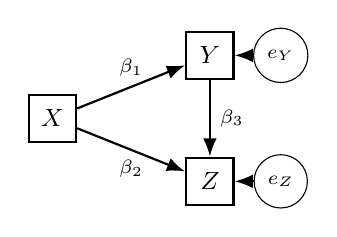
\begin{tikzpicture}[
  >=Latex,
  obs/.style={rectangle, draw=black, thick, minimum size=0.6cm, font=\small},
  err/.style={circle, draw=black, minimum size=0.45cm, font=\scriptsize}
]
  \node[obs] (X) at (0, 0.9) {$X$};
  \node[obs] (Y) at (2.0, 1.7) {$Y$};
  \node[obs] (Z) at (2.0, 0.1) {$Z$};

  \node[err] (eY) at (2.9, 1.7) {$e_Y$};
  \node[err] (eZ) at (2.9, 0.1) {$e_Z$};

  \draw[->, thick] (X) -- node[above, font=\scriptsize] {$\beta_1$} (Y);
  \draw[->, thick] (X) -- node[below, font=\scriptsize] {$\beta_2$} (Z);
  \draw[->, thick] (Y) -- node[right, font=\scriptsize] {$\beta_3$} (Z);
  \draw[->, thick] (eY) -- (Y);
  \draw[->, thick] (eZ) -- (Z);
\end{tikzpicture}
}%
\end{center}

Duota koreliacijų matrica:
\begin{equation*}
    S = \begin{pmatrix} 1 & 0.40 & 0.60 \\ 0.40 & 1 & 0.20 \\ 0.60 & 0.20 & 1 \end{pmatrix}, \quad (r_{XY}=0.4, r_{XZ}=0.6, r_{YZ}=0.2)
\end{equation*}

\textbf{Sprendimas}:
\begin{enumerate}
    \item Kintamajam $Y$: lygtis $Y = \beta_1 X + e_Y$.
    \begin{equation*}
        \text{Cor}(X, Y) = \beta_1 \implies \beta_1 = 0.40
    \end{equation*}
    \item Kintamajam $Z$: lygtis $Z = \beta_2 X + \beta_3 Y + e_Z$.
    \begin{align*}
        \text{Cor}(X, Z) &= \beta_2 + \beta_3 \cdot r_{XY} = \beta_2 + 0.40 \beta_3 = 0.60 \\
        \text{Cor}(Y, Z) &= \beta_2 \cdot r_{XY} + \beta_3 = 0.40 \beta_2 + \beta_3 = 0.20
    \end{align*}
    Taikome greitąją 2x2 formulę ($r = 0.40$, $1 - r^2 = 0.84$):
    \begin{align*}
        \beta_2 &= \frac{0.60 - 0.40(0.20)}{0.84} = \frac{0.52}{0.84} = \frac{13}{21} \approx 0.619 \\
        \beta_3 &= \frac{0.20 - 0.40(0.60)}{0.84} = \frac{-0.04}{0.84} = -\frac{1}{21} \approx -0.048
    \end{align*}
    \item Liekamųjų paklaidų dispersijos:
    \begin{align*}
        \text{Var}(e_Y) &= 1 - \beta_1^2 = 1 - 0.40^2 = 0.84 \\
        \text{Var}(e_Z) &= 1 - (\beta_2 r_{XZ} + \beta_3 r_{YZ}) \\
        &= 1 - (0.619 \cdot 0.60 - 0.048 \cdot 0.20) \\
        &= 1 - 0.3619 = 0.6381
    \end{align*}
    \item Poveikių kintamajam $Z$ išskaidymas:
    \begin{itemize}
        \item $X \to Z$ tiesioginis: $\text{DE} = \beta_2 = 0.619$.
        \item $X \to Z$ netiesioginis per $Y$: $\text{IE} = \beta_1 \cdot \beta_3 = 0.40 \times (-0.048) = -0.019$.
        \item Bendrasis: $\text{TE} = 0.619 - 0.019 = 0.600 = r_{XZ}$!
    \end{itemize}
\end{enumerate}

\section{Dažniausi kontroliniai klausimai ir gudrybės}
\begin{enumerate}
    \item \textbf{Kodėl kelias $A \to C \leftarrow B$ negalioja?}
    Nes rodyklės susiduria smaigaliais ($\to \leftarrow$). Tai yra „collider“ -- informacija per jį neina.
    \item \textbf{Kiek yra nepriklausomų koreliacijų?}
    $k$ kintamiesiems yra $p^* = \frac{k(k-1)}{2}$ porinių koreliacijų. Pvz., $k=4 \implies 6$; $k=5 \implies 10$; $k=6 \implies 15$.
    \item \textbf{Heywood atvejis}: jei apskaičiuota liekamosios paklaidos dispersija gaunama neigiama ($\text{Var}(e) < 0$) arba koreliacija $> 1$, modelis yra blogai specifikuotas arba duomenys netinkami.
    \item \textbf{Kodėl $\chi^2$ reikšmė priklauso nuo $N$?}
    Kadangi $\chi^2 = (N-1) F_{ML}$, esant dideliam $N$ net mažiausi neatitikimai tampa statistiškai reikšmingi ($p < 0.05$). Todėl vertinami RMSEA, CFI, TLI.
\end{enumerate}

\end{multicols*}
\end{document}
